\section{MAGIC Intro}%
\label{sec:magic}
Seit der Entdeckung von Victor Hess der kosmischen Höhenstrahlung 
1912 feiert die Astroteilchenphysik bahnbrechende errungenschaften.
Die Entdeckung der kosmischen Hintergrundstrahlung gilt als beleg des
expandierendes Universum und wirft dennoch weitere Fragen zum frühen Universum auf. 
Die Kosmische Strahlung lässt das erforschen elementarer Bausteine und
Beschlunigungsprozesse zu wovon
einige informationen über ihren Usprung tragen. 
Anhand der kosmischen Botenteilchen wozu neuerdings aus Graviatationswellen
zählen werden Informationen über supernovae, schwarze löcher extrahiert.
\begin{wrapfigure}[13]{o}{0.45\textwidth}
		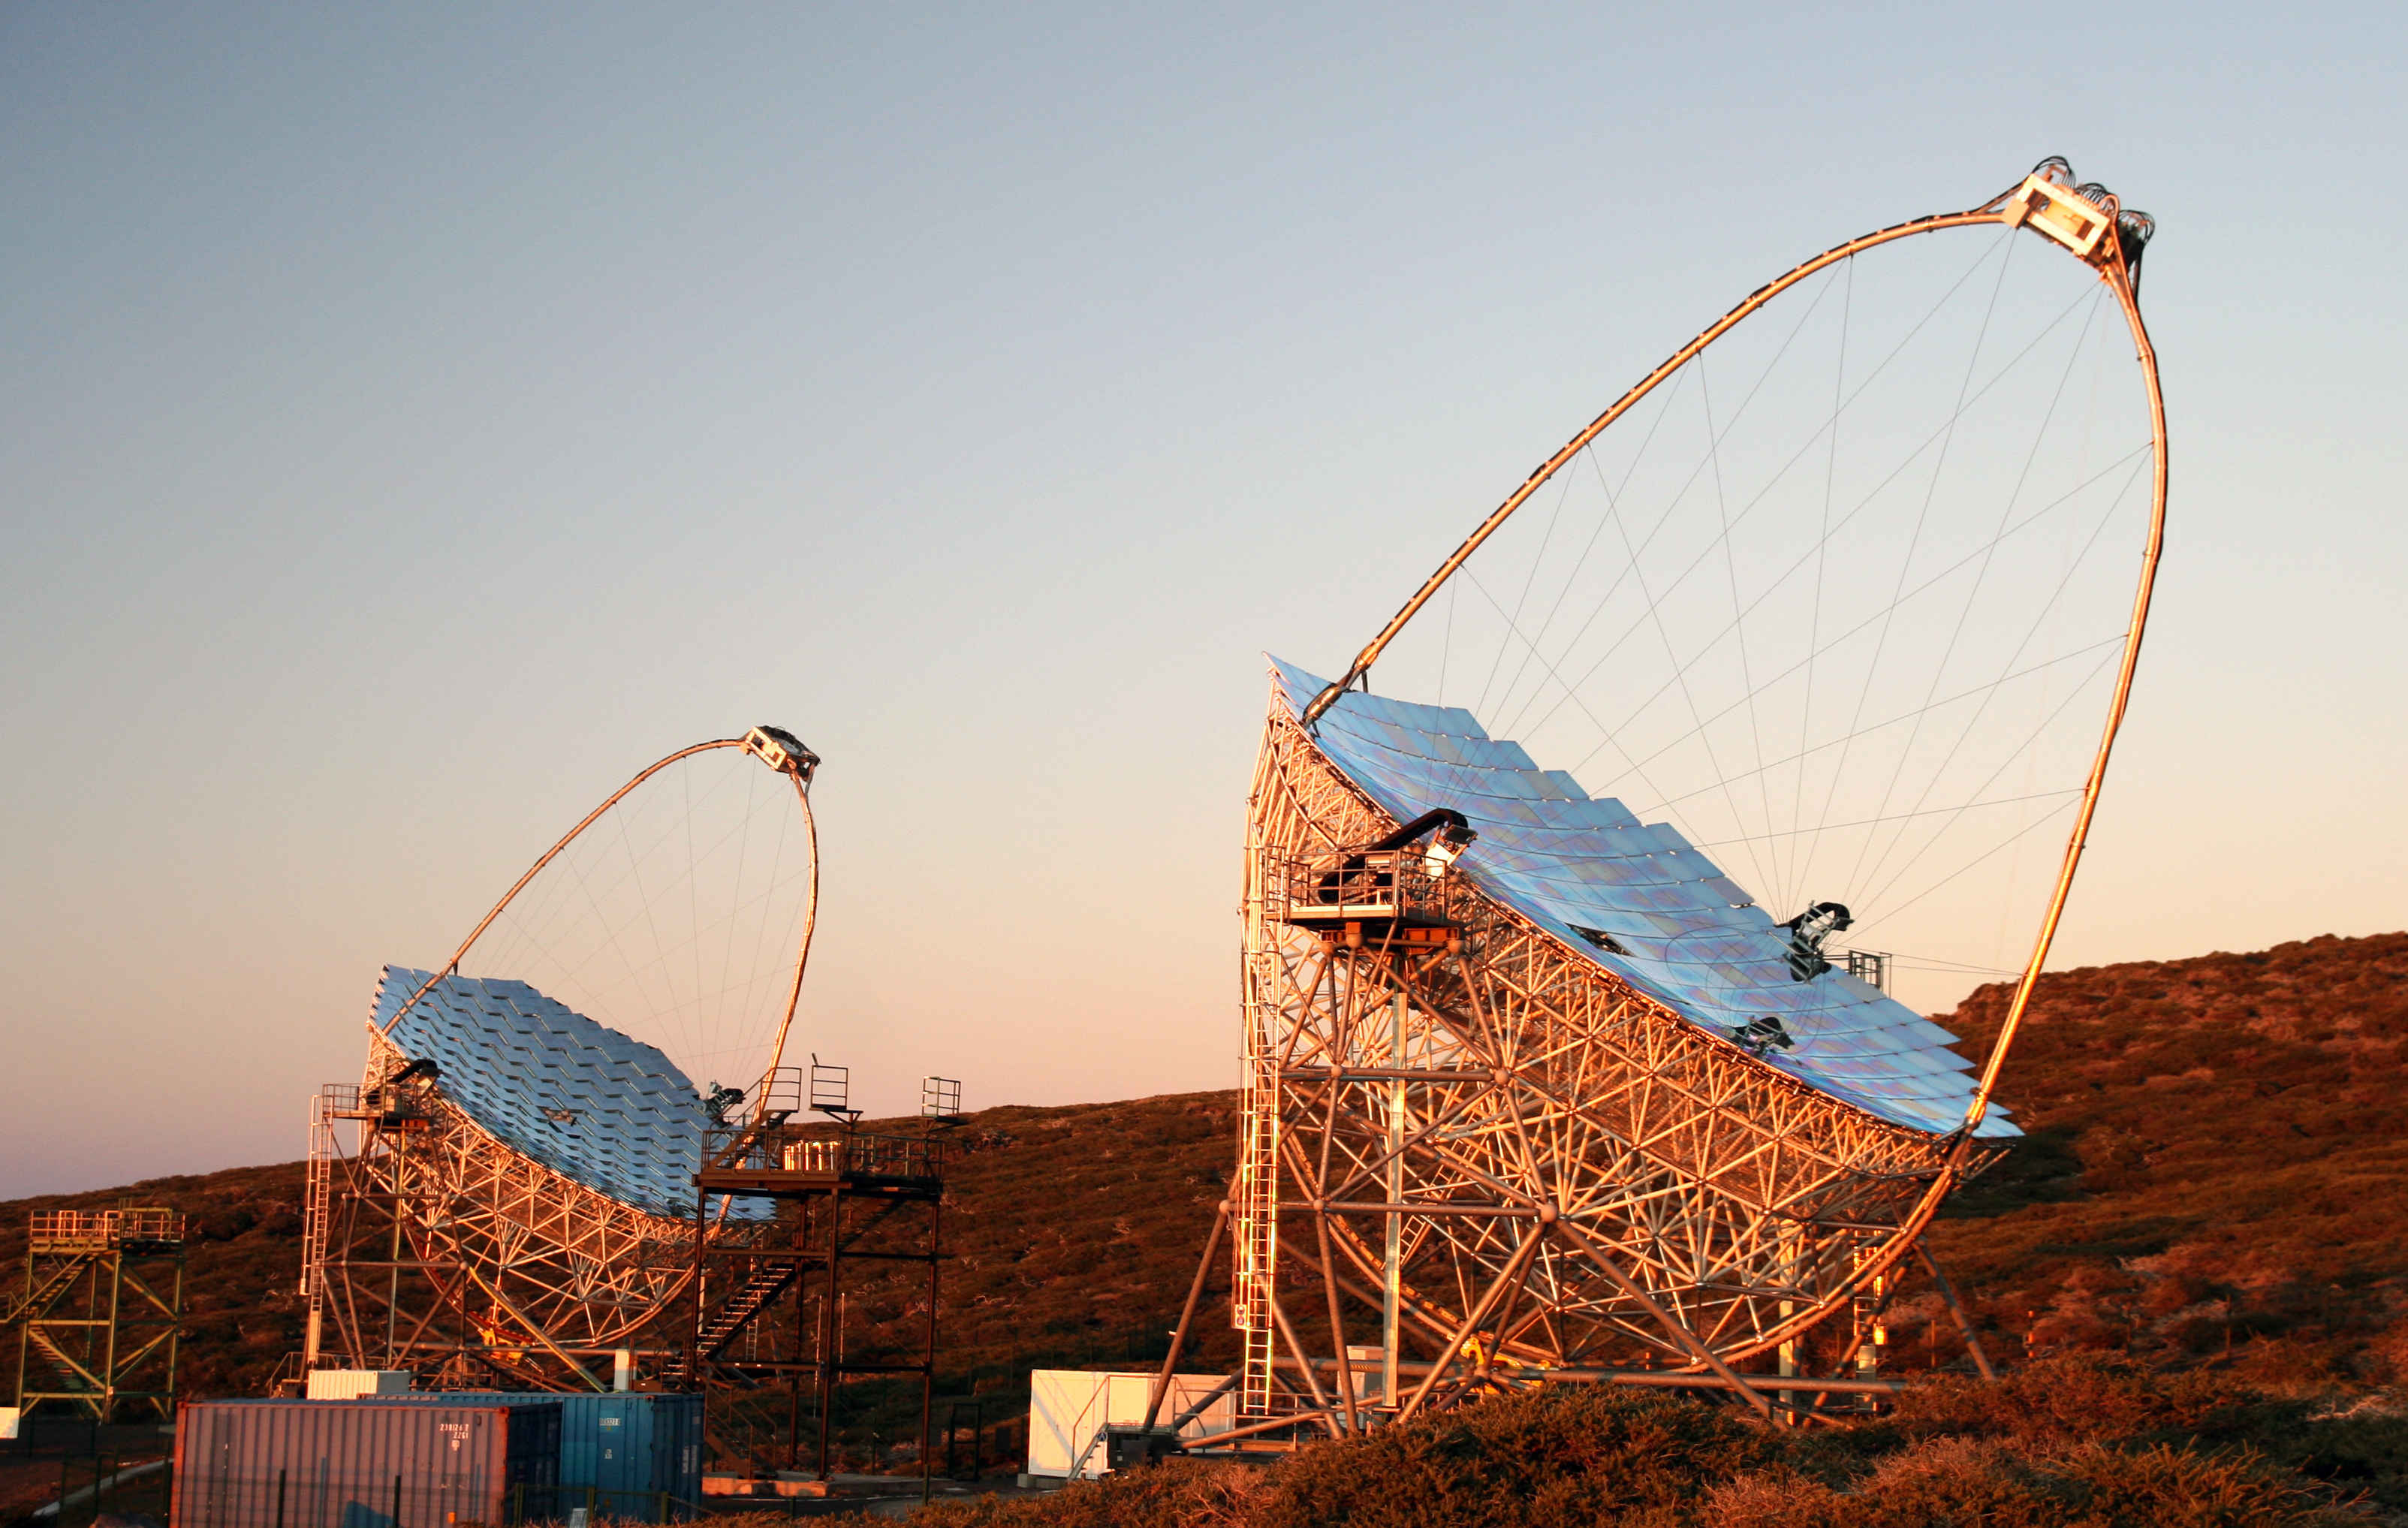
\includegraphics[width=\linewidth]{pictures/magic.JPG}
		\caption{Magic Teleskope in Observationsstellung.}%
		\label{fig:magic}
\end{wrapfigure}
Der Nachweis von hochenergetischer Gammastrahlung ist auf der Erde aufgrund der
Atmosphäre nur indirekt möglich. 
Hochenergetisches Teilchen erzeugen in der Atmosphäre Teilchenschauer, die
aufgrund ihrer relativistischen Geschwindigkeite Tscherenkovlicht abstrahlen.
Magic ist derzeit (16.11.2016) das größte Stereoteleskop mit dem die
Detektion von Tscherenkov-Schauern in einem Energiebereich von
\SI{50}{\giga\electronvolt} bis \SI{50}{\giga\electronvolt} möglich ist.
Es steht auf der Insel La Palma auf einer Höhe von \SI{2200}{\meter}.
Trifft ein Teilchen mit Überlichtgeschwindigkeit in einem Medium, so emittiert
dieses einen Tscherenkov-Kegel. 
Die ultrarelativistischen Teilchen welche auf die Erdatmosphäre treffen
Wechselwirken mit den darin enthaltenen Teilchen beispielsweise über
Bremsstrahlung, Paarerzeugung \ldots und produzieren somit weitere
relativistische Teilchen welche wiederum Tscherenkov kegel erzeugen.

Die dadurch erzeugten Lichtblitze können durch Tscherenkov-Teleskope detektiert
werden.
Die Spiegelfläche von \SI{17}{\meter} Durchmesser besteht aus \num{974} einzelnen
Spiegeln die auf \num{1039} Photo Multiplier Tubes (PMTs) mit einem
Field of View von \SI{3.5}{\degree} abbilden. 

Ziel ist es mit den Teleskopen Gamma-Quellen wie AGNs, Supernovae und
Gasverteilungen in denen viel Sternbildung stattfindet genauer zu observieren. 
Desweiteren wird nach einen indirekten Nachweis nach dunkeler Materie 
Fundamentales Problem geladenen Teilchen jegliche Richtungsinformation verlieren
in kosmologischen Magnetfelder verlieren und somit keine Informationen aus
Quelle rekonstruiert werden. 

\clearpage
